\pageIconAnalysis
\ainfoX{\CTNT}{\href{https://atva-conference.org/2023}
{The 21\stsup International Symposium on Automated Technology for Verification and Analysis (ATVA), 2023}}
{Software artifact: \href{https://doi.org/10.5281/zenodo.7908484}{10.5281/zenodo.7908484}\newline
Citation:~\cite{aubert2023b}\par
\textit{Reproduced with permission from Springer Nature.}}
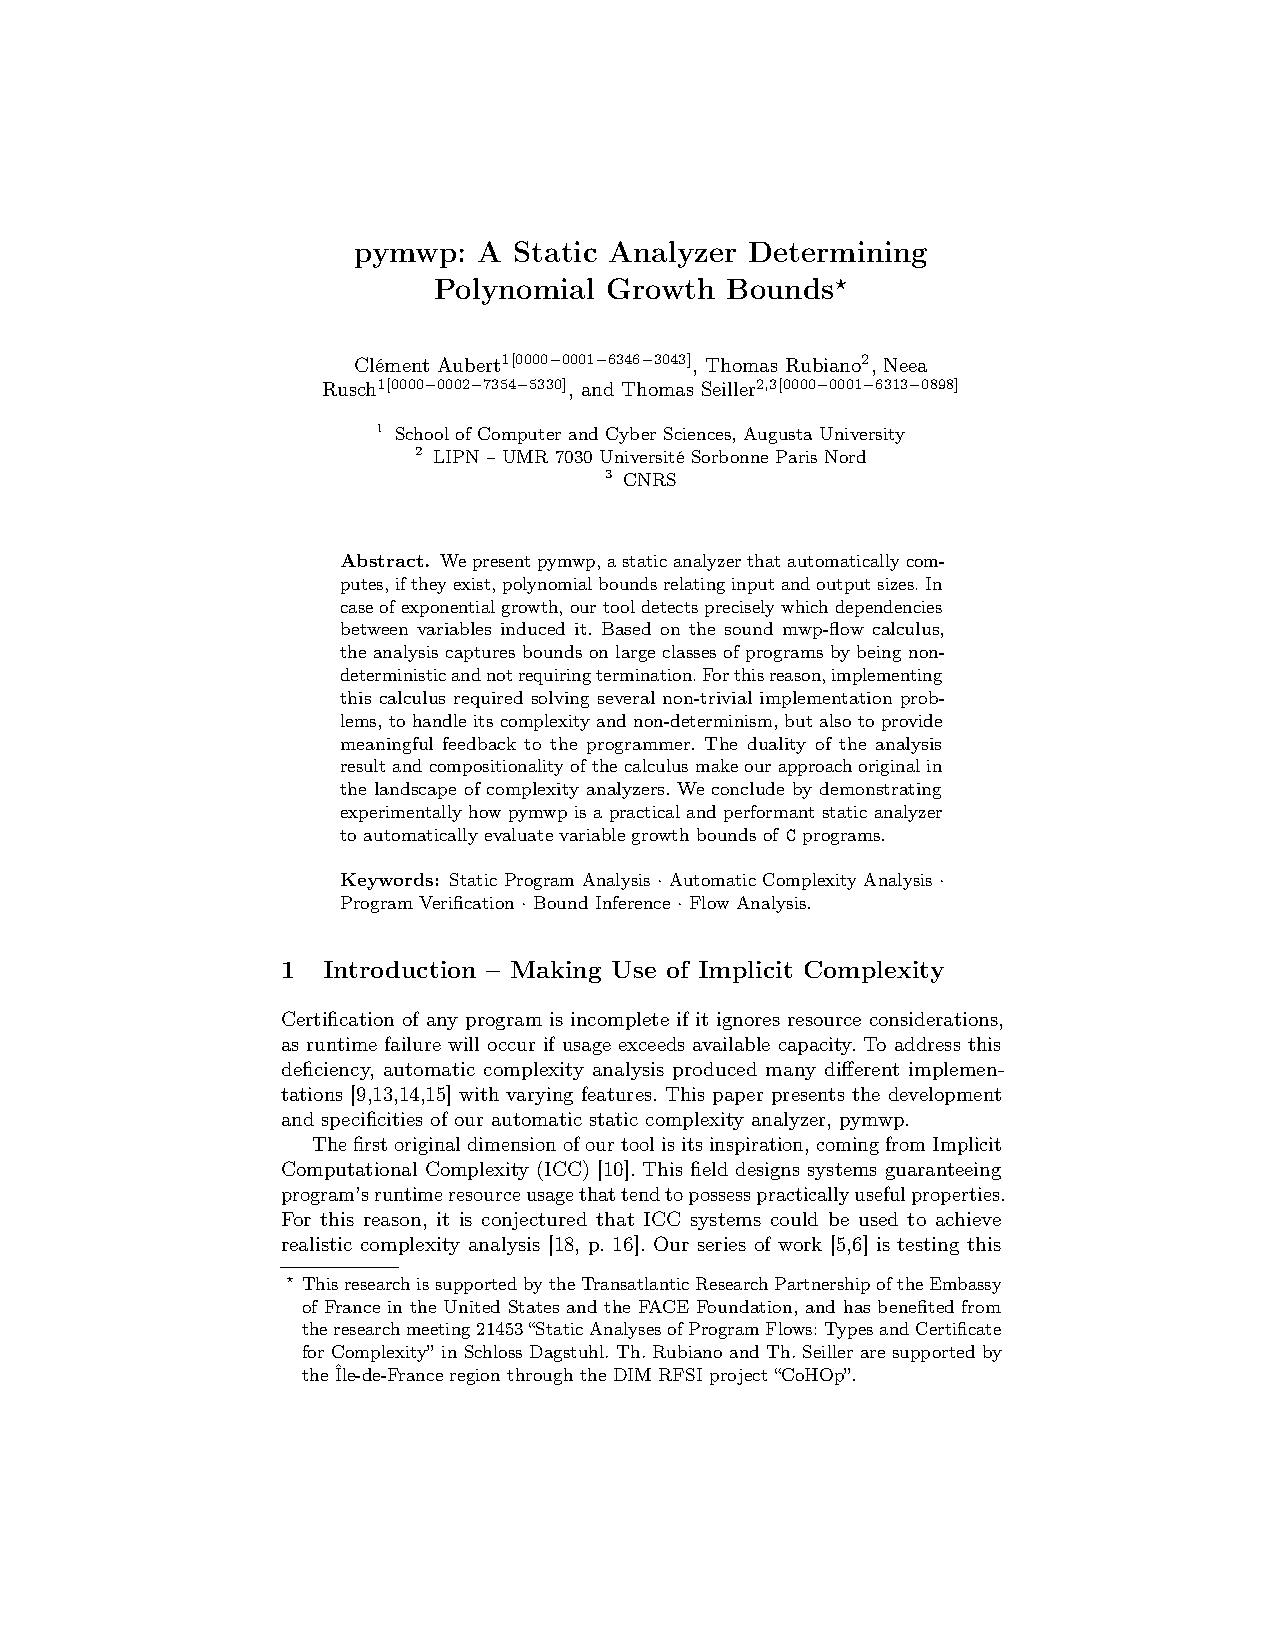
\includepdf[pages={1-},
    addtotoc={
        1,subsection,2,{Introduction -- Making Use of Implicit Complexity},sec:intro,
        3,subsection,2,{Calculating Bounds with mwp-Analysis},sec:idea,
        5,subsection,2,{Technical Overview of pymwp},sec:tool,
        6,subsection,2,{Implementation Advancements},sec:solutions,
        8,subsection,2,{Experimental Evaluation},sec:eval,
        11,subsection,2,{Conclusion},sec:conc},
    addtolist={
        5,table,{Comparison of obtained resource bounds},tab:atva-compare,
        10,table,{Benchmark results},tab:eval,
        10,table,{Examples of obtained bounds},tab:bounds
    }, pagecommand={\thispagestyle{empty}%
    \addtoindexm{C4B}{4,5}
    \addtoindexm{LOOPUS}{4,5}
    \addtoindexm{abstract syntax tree}{5,6}
    \addtoindexm{domain-specific language}{11}
    \addtoindexm{honest polynomial}{3}
    \addtoindexm{intermediate representation}{11}
    \addtoindexm{mwp-bound}{3,8}
    \addtoindexm{nondeterminism}{1,6,7,9,11}
    \addtoindexm{pycparser}{6}
    \addtoindexm{pymwp}{1,2,4,5,6,7,8,9,11}
    \addtoindexm{mwp-matrix}{9}
    \addtoindexm{choice vector}{8}
    \addtosymbolsm{Xprime}{2,3,4,5,9}
    \addtosymbolsm{hp}{3}
    \addtosymbolsm{infty}{3,4,7,8,9,10}
    \addtosymbolsm{m}{3}
    \addtosymbolsm{p}{3}
    \addtosymbolsm{w}{3}
    \addtosymbolsm{zero}{3,5,10}
    }]{pdf/pubs_atva.2023.pdf}